\documentclass[border=6pt]{standalone}
\usepackage{tikz}
\usepackage[edges]{forest}
\usetikzlibrary{arrows.meta,positioning,calc,decorations.pathreplacing,shapes.geometric}
\begin{document}
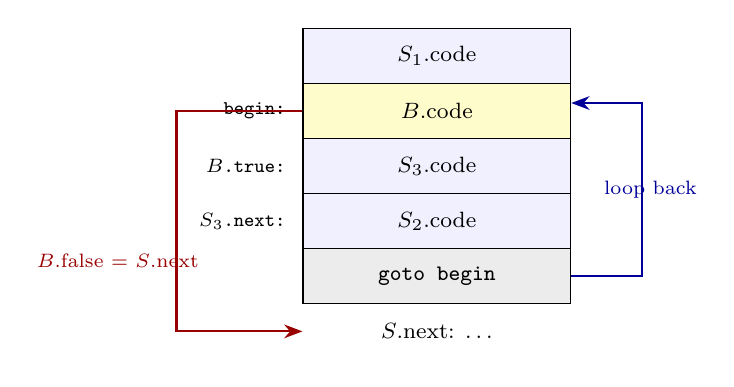
\begin{tikzpicture}[>=Stealth,font=\small,
 cell/.style={draw,minimum width=3.4cm,minimum height=0.7cm,align=center,font=\footnotesize},
 lab/.style={font=\scriptsize\ttfamily,anchor=east}]
\node[cell,fill=blue!6] (s1) at (0,0) {$S_1$.code};
\node[cell,fill=yellow!20] (b) at (0,-0.7) {$B$.code};
\node[cell,fill=blue!6] (s3) at (0,-1.4) {$S_3$.code};
\node[cell,fill=blue!6] (s2) at (0,-2.1) {$S_2$.code};
\node[cell,fill=gray!15] (g) at (0,-2.8) {\texttt{goto begin}};
\node[cell,draw=none] (nx) at (0,-3.5) {$S$.next: $\ldots$};
\node[lab] at (-1.8,-0.7) {begin:}; \node[lab] at (-1.8,-1.4) {$B$.true:}; \node[lab] at (-1.8,-2.1) {$S_3$.next:};
\draw[->,thick,blue!60!black] (g.east) -- ++(0.9,0) |- ([yshift=0.1cm]b.east);
\draw[->,thick,red!60!black] (b.west) -- ++(-1.6,0) |- (nx.west);
\node[font=\scriptsize,anchor=west,blue!60!black] at (2.0,-1.7) {loop back};
\node[font=\scriptsize,anchor=east,red!60!black] at (-2.9,-2.6) {$B$.false $=$ $S$.next};
\end{tikzpicture}
\end{document}
